% ==============================================================================
% BỘ ĐỀ THAM KHẢO TUYỂN SINH 10 NĂM HỌC 2026-2027 SỞ GD&ĐT TP.HCM
% ĐỢT 11: CỤM 8 - ĐỀ 1 & CỤM 8 - ĐỀ 2 (14 CÂU TỰ LUẬN)
% ==============================================================================

% ==============================================================================
% CỤM 8 - ĐỀ THAM KHẢO 1 (Đề số 22)
% ==============================================================================

\begin{bt}%[9D6H18-2]
% nguon: Đề tham khảo Tuyển sinh 10 năm học 2026-2027 Sở GD&ĐT TP.HCM - Cụm 8 Đề 1, Bài 1
	Cho hàm số $y = -\dfrac{1}{2}x^2$ có đồ thị là parabol $(P)$.
	\begin{enumerate}[a)]
		\item Vẽ đồ thị $(P)$ của hàm số trên.
		\item Tìm tọa độ các điểm $M$ thuộc $(P)$ (khác gốc tọa độ $O$) có hoành độ bằng tung độ.
	\end{enumerate}
	\loigiai{
		\begin{enumerate}[a)]
			\item Bảng giá trị tương ứng giữa $x$ và $y$ của parabol $(P)\colon y = -\dfrac{1}{2}x^2$:
			\begin{center}
				\begin{tabular}{|c|c|c|c|c|c|}
					\hline
					$x$ & $-2$ & $-1$ & $0$ & $1$ & $2$ \\
					\hline
					$y = -\dfrac{1}{2}x^2$ & $-2$ & $-0{,}5$ & $0$ & $-0{,}5$ & $-2$ \\
					\hline
				\end{tabular}
			\end{center}
			Đồ thị $(P)$ là một parabol đi qua gốc tọa độ $O(0;0)$, nằm phía dưới trục hoành và nhận trục tung $Oy$ làm trục đối xứng.
			\begin{center}
				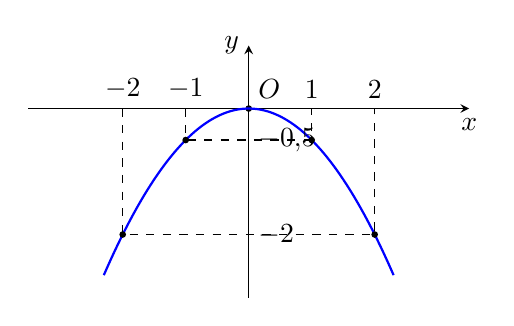
\begin{tikzpicture}[>=stealth, scale=0.8]
					\draw[->] (-3.5,0) -- (3.5,0) node[below] {$x$};
					\draw[->] (0,-3) -- (0,1) node[left] {$y$};
					\fill (0,0) circle (1.5pt) node[above right] {$O$};
					\draw[smooth, samples=100, domain=-2.3:2.3, thick, color=blue] plot(\x, {-1/2*(\x)^2});
					\draw[dashed] (-2,0) node[above] {$-2$} -- (-2,-2) -- (0,-2) node[right] {$-2$} -- (2,-2) -- (2,0) node[above] {$2$};
					\draw[dashed] (-1,0) node[above] {$-1$} -- (-1,-0.5) -- (0,-0.5) node[right] {$-0{,}5$} -- (1,-0.5) -- (1,0) node[above] {$1$};
					\fill (-2,-2) circle (1.5pt) (2,-2) circle (1.5pt) (-1,-0.5) circle (1.5pt) (1,-0.5) circle (1.5pt);
				\end{tikzpicture}
			\end{center}
			\item Vì điểm $M$ có hoành độ bằng tung độ nên ta có:
			$$y = x.$$
			Mặt khác $M \in (P)$ nên ta có phương trình:
			$$x = -\dfrac{1}{2}x^2 \iff \dfrac{1}{2}x^2 + x = 0 \iff x\left(\dfrac{1}{2}x + 1\right) = 0 \iff \left[\begin{aligned} &x = 0 \\ &x = -2. \end{aligned}\right.$$
			Vì $M$ khác gốc tọa độ $O$ nên $x \neq 0$, suy ra $x = -2$.
			
			Với $x = -2 \implies y = -2$.
			
			Vậy tọa độ điểm cần tìm là $M(-2; -2)$.
		\end{enumerate}
	}
\end{bt}

\begin{bt}%[9D6H20-2]
% nguon: Đề tham khảo Tuyển sinh 10 năm học 2026-2027 Sở GD&ĐT TP.HCM - Cụm 8 Đề 1, Bài 2
	Cho phương trình $x^2 - 4x + 2 = 0$.
	\begin{enumerate}[a)]
		\item Chứng minh phương trình trên luôn có hai nghiệm phân biệt $x_1, x_2$.
		\item Không giải phương trình, hãy tính giá trị của biểu thức:
		$$A = (x_1 - x_2)^2 - x_1 - x_2.$$
	\end{enumerate}
	\loigiai{
		\begin{enumerate}[a)]
			\item Phương trình $x^2 - 4x + 2 = 0$ có $a = 1, b = -4, c = 2$.
			
			Ta có:
			$$\Delta' = (-2)^2 - 1 \cdot 2 = 4 - 2 = 2 > 0.$$
			Vì $\Delta' > 0$ nên phương trình luôn có hai nghiệm phân biệt $x_1, x_2$.
			\item Theo định lí Viète, ta có:
			$$\begin{cases} x_1 + x_2 = 4 \\ x_1 x_2 = 2. \end{cases}$$
			Ta có:
			$$x_1^2 + x_2^2 = (x_1 + x_2)^2 - 2x_1 x_2 = 4^2 - 2 \cdot 2 = 16 - 4 = 12.$$
			Biến đổi biểu thức $A$:
			$$A = (x_1 - x_2)^2 - (x_1 + x_2) = (x_1^2 + x_2^2) - 2x_1 x_2 - (x_1 + x_2).$$
			Thay các giá trị vào biểu thức $A$, ta được:
			$$A = 12 - 2 \cdot 2 - 4 = 12 - 4 - 4 = 4.$$
			Vậy $A = 4$.
		\end{enumerate}
	}
\end{bt}

\begin{bt}%[9D8H26-3]
% nguon: Đề tham khảo Tuyển sinh 10 năm học 2026-2027 Sở GD&ĐT TP.HCM - Cụm 8 Đề 1, Bài 3
	Số lượng máy tính để bàn và máy tính xách tay bán ra trong $6$ tháng cuối năm của một công ty được thống kê như sau: Tháng 7 (80 để bàn, 38 xách tay); Tháng 8 (41 để bàn, 27 xách tay); Tháng 9 (23 để bàn, 49 xách tay); Tháng 10 (20 để bàn, 64 xách tay); Tháng 11 (14 để bàn, 55 xách tay); Tháng 12 (7 để bàn, 76 xách tay).
	\begin{enumerate}[a)]
		\item Trong $6$ tháng cuối năm, tháng nào có sự chênh lệch giữa số lượng máy tính xách tay và máy tính để bàn bán ra là nhiều nhất?
		\item Chọn ngẫu nhiên $1$ tháng trong $6$ tháng cuối năm. Tính xác suất của các biến cố sau:
		\begin{itemize}
			\item Biến cố $A$: ``Tháng được chọn có số lượng máy tính để bàn bán được ít nhất $20$ cái''.
			\item Biến cố $B$: ``Tháng được chọn có tỉ lệ giữa số lượng máy tính xách tay và máy tính để bàn lớn hơn $2$''.
		\end{itemize}
	\end{enumerate}
	\loigiai{
		\begin{enumerate}[a)]
			\item Bảng thống kê độ chênh lệch số lượng bán giữa máy tính xách tay và máy tính để bàn qua các tháng:
			\begin{center}
				\begin{tabular}{|l|c|c|c|c|c|c|}
					\hline
					\textbf{Tháng} & Tháng 7 & Tháng 8 & Tháng 9 & Tháng 10 & Tháng 11 & Tháng 12 \\
					\hline
					\textbf{Máy tính để bàn} & 80 & 41 & 23 & 20 & 14 & 7 \\
					\hline
					\textbf{Máy tính xách tay} & 38 & 27 & 49 & 64 & 55 & 76 \\
					\hline
					\textbf{Độ chênh lệch} & 42 & 14 & 26 & 44 & 41 & 69 \\
					\hline
				\end{tabular}
			\end{center}
			Độ chênh lệch lớn nhất là $69$ cái vào Tháng 12.
			
			Vậy Tháng 12 có sự chênh lệch nhiều nhất giữa số lượng máy tính xách tay và để bàn.
			\item Không gian mẫu gồm $6$ tháng nên $n(\Omega) = 6$.
			\begin{itemize}
				\item Các tháng có số lượng máy tính để bàn bán được ít nhất $20$ cái là: Tháng 7 (80 cái), Tháng 8 (41 cái), Tháng 9 (23 cái), Tháng 10 (20 cái).
				
				Số kết quả thuận lợi cho biến cố $A$ là $n(A) = 4$.
				
				Xác suất của biến cố $A$ là:
				$$P(A) = \dfrac{n(A)}{n(\Omega)} = \dfrac{4}{6} = \dfrac{2}{3}.$$
				\item Xét tỉ số $\dfrac{\text{Máy tính xách tay}}{\text{Máy tính để bàn}}$ ở từng tháng:
				- Tháng 7: $\dfrac{38}{80} < 1$;
				- Tháng 8: $\dfrac{27}{41} < 1$;
				- Tháng 9: $\dfrac{49}{23} \approx 2{,}13 > 2$ (thỏa mãn);
				- Tháng 10: $\dfrac{64}{20} = 3{,}2 > 2$ (thỏa mãn);
				- Tháng 11: $\dfrac{55}{14} \approx 3{,}93 > 2$ (thỏa mãn);
				- Tháng 12: $\dfrac{76}{7} \approx 10{,}86 > 2$ (thỏa mãn).
				
				Có $4$ tháng có tỉ lệ lớn hơn $2$ là: Tháng 9, Tháng 10, Tháng 11, Tháng 12.
				
				Số kết quả thuận lợi cho biến cố $B$ là $n(B) = 4$.
				
				Xác suất của biến cố $B$ là:
				$$P(B) = \dfrac{n(B)}{n(\Omega)} = \dfrac{4}{6} = \dfrac{2}{3}.$$
			\end{itemize}
		\end{enumerate}
	}
\end{bt}

\begin{bt}%[9D6V21-3]
% nguon: Đề tham khảo Tuyển sinh 10 năm học 2026-2027 Sở GD&ĐT TP.HCM - Cụm 8 Đề 1, Bài 4
	Một mảnh vườn hình chữ nhật có chiều rộng bằng $a\text{ (m)}$, chiều dài hơn chiều rộng $6\text{ m}$. Người ta làm một lối đi hình chữ thập rộng $x\text{ (m)}$ gồm một dải dọc và một dải ngang (với $a > 0$ và $0 < x < a$). Phần đất còn lại ở bốn góc được dùng để trồng rau.
	\begin{enumerate}[a)]
		\item Hãy viết biểu thức thu gọn theo $x$ và $a$ biểu thị diện tích phần đất còn lại dùng để trồng rau.
		\item Tính diện tích đất dùng để trồng rau khi $a = 30\text{ m}$ và $x = 1\text{ m}$.
	\end{enumerate}
	\loigiai{
		\begin{enumerate}[a)]
			\item Chiều rộng ban đầu của mảnh vườn là $a\text{ (m)}$.
			
			Chiều dài ban đầu của mảnh vườn là $a + 6\text{ (m)}$.
			
			Khi làm lối đi chữ thập có bề rộng $x\text{ (m)}$, tổng chiều rộng của phần đất trồng rau còn lại là:
			$$a - x\text{ (m)}.$$
			Tổng chiều dài của phần đất trồng rau còn lại là:
			$$(a + 6) - x = a - x + 6\text{ (m)}.$$
			Diện tích phần đất còn lại dùng để trồng rau là:
			$$S = (a - x)(a - x + 6) = (a - x)^2 + 6(a - x)\text{ (m}^2).$$
			\item Thay $a = 30\text{ m}$ và $x = 1\text{ m}$ vào biểu thức $S$, ta được:
			$$S = (30 - 1)(30 - 1 + 6) = 29 \cdot 35 = 1015\text{ (m}^2).$$
			Vậy diện tích đất dùng để trồng rau là $1015\text{ m}^2$.
		\end{enumerate}
	}
\end{bt}

\begin{bt}%[9H0V31-3]
% nguon: Đề tham khảo Tuyển sinh 10 năm học 2026-2027 Sở GD&ĐT TP.HCM - Cụm 8 Đề 1, Bài 5
	Cho một khối xốp hình trụ có bán kính đáy $R = 10\text{ cm}$ và chiều cao $h = OO' = 8\text{ cm}$. Người ta gọt bỏ phần xung quanh của khối xốp hình trụ để tạo thành một khối xốp hình nón có đỉnh là $O'$ và đáy là hình tròn đáy $(O; R)$ của hình trụ.
	\begin{enumerate}[a)]
		\item Tính thể tích phần xốp bị gọt bỏ đi theo $\pi$.
		\item Nếu bán kính đáy $R$ của hình trụ giảm đi một nửa và giữ nguyên chiều cao thì thể tích của hình trụ thay đổi như thế nào?
	\end{enumerate}
	\loigiai{
		\begin{enumerate}[a)]
			\item Thể tích của khối xốp hình trụ ban đầu là:
			$$V_{\text{trụ}} = \pi R^2 h = \pi \cdot 10^2 \cdot 8 = 800\pi\text{ (cm}^3).$$
			Thể tích của khối xốp hình nón sau khi gọt là:
			$$V_{\text{nón}} = \dfrac{1}{3}\pi R^2 h = \dfrac{1}{3}\pi \cdot 10^2 \cdot 8 = \dfrac{800\pi}{3}\text{ (cm}^3).$$
			Thể tích phần xốp bị gọt bỏ đi là:
			$$V_{\text{bỏ}} = V_{\text{trụ}} - V_{\text{nón}} = 800\pi - \dfrac{800\pi}{3} = \dfrac{1600\pi}{3}\text{ (cm}^3).$$
			\item Thể tích hình trụ ban đầu là $V_1 = \pi R^2 h$.
			
			Khi bán kính giảm một nửa thì bán kính mới là $R' = \dfrac{R}{2}$.
			
			Thể tích hình trụ lúc sau là:
			$$V_2 = \pi (R')^2 h = \pi \left(\dfrac{R}{2}\right)^2 h = \dfrac{\pi R^2 h}{4} = \dfrac{1}{4}V_1.$$
			Vậy thể tích hình trụ giảm đi $4$ lần.
		\end{enumerate}
	}
\end{bt}

\begin{bt}%[9D1H3-4]
% nguon: Đề tham khảo Tuyển sinh 10 năm học 2026-2027 Sở GD&ĐT TP.HCM - Cụm 8 Đề 1, Bài 6
	Có hai thùng chứa nước. Người ta đổ nước từ thùng thứ nhất sang thùng thứ hai một lượng nước bằng lượng nước thùng thứ hai đang có; tiếp tục đổ nước từ thùng thứ hai sang thùng thứ nhất một lượng nước bằng lượng nước thùng thứ nhất đang có; sau đó lại đổ nước từ thùng thứ nhất sang thùng thứ hai một lượng nước bằng lượng nước thùng thứ hai đang có. Cuối cùng, cả hai thùng đều chứa đúng $160$ lít nước. Hỏi lúc đầu mỗi thùng chứa bao nhiêu lít nước?
	\loigiai{
		Gọi $x$ (lít) là lượng nước ban đầu của thùng thứ nhất ($x > 0$).
		
		Gọi $y$ (lít) là lượng nước ban đầu của thùng thứ hai ($y > 0$).
		\begin{itemize}
			\item \textbf{Lần đổ thứ nhất:} Đổ từ thùng 1 sang thùng 2 lượng nước bằng $y$ lít:
			- Thùng 1 còn: $x - y$ (lít).
			- Thùng 2 có: $y + y = 2y$ (lít).
			\item \textbf{Lần đổ thứ hai:} Đổ từ thùng 2 sang thùng 1 lượng nước bằng $x - y$ lít:
			- Thùng 1 có: $(x - y) + (x - y) = 2x - 2y$ (lít).
			- Thùng 2 còn: $2y - (x - y) = 3y - x$ (lít).
			\item \textbf{Lần đổ thứ ba:} Đổ từ thùng 1 sang thùng 2 lượng nước bằng $3y - x$ lít:
			- Thùng 1 còn: $(2x - 2y) - (3y - x) = 3x - 5y$ (lít).
			- Thùng 2 có: $(3y - x) + (3y - x) = 6y - 2x$ (lít).
		\end{itemize}
		Sau ba lần đổ, mỗi thùng đều có $160$ lít nước nên ta có hệ phương trình:
		$$\begin{cases} 3x - 5y = 160 \\ 6y - 2x = 160 \end{cases} \iff \begin{cases} 3x - 5y = 160 \\ -2x + 6y = 160 \end{cases} \iff \begin{cases} 6x - 10y = 320 \\ -6x + 18y = 480 \end{cases} \iff \begin{cases} 8y = 800 \\ 3x = 160 + 5y \end{cases} \iff \begin{cases} y = 100\text{ (nhận)} \\ x = 220\text{ (nhận)}. \end{cases}$$
		Vậy lúc đầu thùng thứ nhất chứa $220$ lít nước và thùng thứ hai chứa $100$ lít nước.
	}
\end{bt}

\begin{bt}%[9H9C29-3]
% nguon: Đề tham khảo Tuyển sinh 10 năm học 2026-2027 Sở GD&ĐT TP.HCM - Cụm 8 Đề 1, Bài 7
	Cho đường tròn $(O; R)$ có đường kính $AC$. Trên $(O)$ lấy điểm $D$ sao cho $AD = R$. Tiếp tuyến tại $A$ của $(O)$ cắt tia $CD$ tại $B$. Dựng $AE \perp BO$ tại $E$.
	\begin{enumerate}[a)]
		\item Chứng minh $\widehat{ADC} = 90^\circ$ và tứ giác $ABDE$ nội tiếp đường tròn.
		\item Tia $DE$ cắt $(O)$ tại $K$ ($K \neq D$), vẽ đường kính $KH$ của $(O)$. Chứng minh $\widehat{ADE} = \widehat{OAE}$ và ba điểm $A, E, H$ thẳng hàng.
		\item Kẻ $OF \perp BC$ tại $F$, tia $OF$ cắt $AH$ tại $I$, tia $ID$ cắt $AB$ tại $J$. Chứng minh $IJ$ là tiếp tuyến của $(O)$ và tính diện tích tam giác $IJA$ theo $R$.
	\end{enumerate}
	\loigiai{
		\begin{center}
			\begin{tikzpicture}[>=stealth, scale=1]
				\coordinate (O) at (0,0);
				\def\r{2.2}
				\coordinate (A) at (0,\r);
				\coordinate (C) at (0,-\r);
				\draw (O) circle (\r);
				\draw (A) -- (C);
				\coordinate (D) at (30:\r);
				\draw (A) -- (D);
				\draw (C) -- (D);
				\coordinate (B) at (2.54,\r);
				\draw (A) -- (B);
				\draw (D) -- (B);
				\draw (O) -- (B);
				\coordinate (E) at ($(O)!(A)!(B)$);
				\draw (A) -- (E);
				\draw (D) -- (E);
				\node at (O) [left] {$O$};
				\node at (A) [above left] {$A$};
				\node at (C) [below] {$C$};
				\node at (D) [above right] {$D$};
				\node at (B) [above right] {$B$};
				\node at (E) [below] {$E$};
				\fill (O) circle (1.5pt) (A) circle (1.5pt) (C) circle (1.5pt) (D) circle (1.5pt) (B) circle (1.5pt) (E) circle (1.5pt);
			\end{tikzpicture}
		\end{center}
		\begin{enumerate}[a)]
			\item Vì $\widehat{ADC}$ là góc nội tiếp chắn nửa đường tròn đường kính $AC$ nên $\widehat{ADC} = 90^\circ$.
			
			Suy ra $AD \perp BC \implies \widehat{ADB} = 90^\circ$.
			
			Vì $AE \perp BO$ tại $E$ nên $\widehat{AEB} = 90^\circ$.
			
			Tứ giác $ABDE$ có $\widehat{ADB} = \widehat{AEB} = 90^\circ$, do đó hai đỉnh kề nhau $D$ và $E$ cùng nhìn đoạn $AB$ dưới góc vuông.
			
			Suy ra tứ giác $ABDE$ nội tiếp đường tròn đường kính $AB$.
			\item Tứ giác $ABDE$ nội tiếp nên $\widehat{ADE} = \widehat{ABE}$ (hai góc nội tiếp cùng chắn cung $AE$).
			
			Tam giác $OAB$ vuông tại $A$ có đường cao $AE$, do đó $\widehat{ABE} = \widehat{OAE}$ (cùng phụ với $\widehat{AOB}$).
			
			Suy ra $\widehat{ADE} = \widehat{OAE}$.
			
			Trong đường tròn $(O)$, ta có $\widehat{ADK} = \widehat{AHK}$ (hai góc nội tiếp cùng chắn cung $AK$).
			
			Vì $D, E, K$ thẳng hàng nên $\widehat{ADK} = \widehat{ADE} = \widehat{OAE} \implies \widehat{OAE} = \widehat{AHK}$.
			
			Mặt khác tam giác $OAH$ cân tại $O$ (vì $OA = OH = R$) nên $\widehat{OAH} = \widehat{OHA} = \widehat{AHK}$.
			
			Suy ra $\widehat{OAE} = \widehat{OAH}$, do đó hai tia $AE$ và $AH$ trùng nhau.
			
			Vậy ba điểm $A, E, H$ thẳng hàng.
			\item Vì $AD = OA = OD = R$ nên tam giác $AOD$ đều $\implies \widehat{AOD} = 60^\circ$.
			
			Ta có $OF \perp BC$ và $AD \perp BC$ nên $OF \parallel AD \implies \widehat{FOC} = \widehat{DAC} = 60^\circ$ (đồng vị).
			
			Do đó $\widehat{AOF} = 180^\circ - \widehat{FOC} = 120^\circ$.
			
			Vì $\widehat{AOD} = 60^\circ = \dfrac{1}{2}\widehat{AOF}$ nên tia $OD$ là tia phân giác của $\widehat{AOF}$ (tức $\widehat{AOI}$).
			
			Xét $\Delta OAJ$ và $\Delta ODJ$ có $OA = OD = R$, $OJ$ chung và $\widehat{AOJ} = \widehat{DOJ} = 30^\circ$.
			
			Do đó $\Delta OAJ = \Delta ODJ\text{ (c-g-c)} \implies \widehat{ODJ} = \widehat{OAJ} = 90^\circ$.
			
			Suy ra $OD \perp IJ$ tại $D \in (O)$, nên $IJ$ là tiếp tuyến của $(O)$.
			
			Trong tam giác vuông $OAJ$ tại $A$:
			$$AJ = OA \cdot \tan\widehat{AOJ} = R \cdot \tan 30^\circ = \dfrac{R\sqrt{3}}{3}.$$
			Điểm $I$ là giao điểm của $OF$ và $AH$, ta có đường thẳng qua $I$ vuông góc với $AC$ tại $C$, suy ra khoảng cách từ $I$ đến đường thẳng $AB$ bằng $AC = 2R$.
			
			Chiều cao hạ từ $I$ xuống cạnh $AJ$ (nằm trên $AB$) là $h = AC = 2R$.
			
			Diện tích tam giác $IJA$ là:
			$$S_{IJA} = \dfrac{1}{2} \cdot AJ \cdot h = \dfrac{1}{2} \cdot \dfrac{R\sqrt{3}}{3} \cdot 2R = \dfrac{R^2\sqrt{3}}{3}.$$
		\end{enumerate}
	}
\end{bt}

% ==============================================================================
% CỤM 8 - ĐỀ THAM KHẢO 2 (Đề số 23)
% ==============================================================================

\begin{bt}%[9D6H18-2]
% nguon: Đề tham khảo Tuyển sinh 10 năm học 2026-2027 Sở GD&ĐT TP.HCM - Cụm 8 Đề 2, Bài 1
	Cho hàm số $y = -\dfrac{x^2}{2}$ có đồ thị là parabol $(P)$.
	\begin{enumerate}[a)]
		\item Vẽ đồ thị $(P)$ của hàm số trên mặt phẳng tọa độ $Oxy$.
		\item Tìm các điểm $M$ thuộc đồ thị $(P)$ sao cho tung độ và hoành độ là hai số đối nhau.
	\end{enumerate}
	\loigiai{
		\begin{enumerate}[a)]
			\item Bảng giá trị của hàm số $y = -\dfrac{x^2}{2}$:
			\begin{center}
				\begin{tabular}{|c|c|c|c|c|c|}
					\hline
					$x$ & $-4$ & $-2$ & $0$ & $2$ & $4$ \\
					\hline
					$y = -\dfrac{x^2}{2}$ & $-8$ & $-2$ & $0$ & $-2$ & $-8$ \\
					\hline
				\end{tabular}
			\end{center}
			Đồ thị $(P)$ là một parabol đi qua gốc tọa độ $O(0;0)$, nằm phía dưới trục hoành và nhận trục tung $Oy$ làm trục đối xứng.
			\begin{center}
				\begin{tikzpicture}[>=stealth, scale=0.7]
					\draw[->] (-5,0) -- (5,0) node[below] {$x$};
					\draw[->] (0,-9) -- (0,1.5) node[left] {$y$};
					\fill (0,0) circle (1.5pt) node[above right] {$O$};
					\draw[smooth, samples=100, domain=-4.2:4.2, thick, color=blue] plot(\x, {-1/2*(\x)^2});
					\draw[dashed] (-4,0) node[above] {$-4$} -- (-4,-8) -- (0,-8) node[right] {$-8$} -- (4,-8) -- (4,0) node[above] {$4$};
					\draw[dashed] (-2,0) node[above] {$-2$} -- (-2,-2) -- (0,-2) node[right] {$-2$} -- (2,-2) -- (2,0) node[above] {$2$};
					\fill (-4,-8) circle (1.5pt) (4,-8) circle (1.5pt) (-2,-2) circle (1.5pt) (2,-2) circle (1.5pt);
				\end{tikzpicture}
			\end{center}
			\item Vì tung độ và hoành độ là hai số đối nhau nên ta có phương trình:
			$$y = -x.$$
			Mặt khác điểm đó thuộc $(P)$ nên:
			$$-\dfrac{x^2}{2} = -x \iff x^2 - 2x = 0 \iff x(x - 2) = 0 \iff \left[\begin{aligned} &x = 0 \\ &x = 2. \end{aligned}\right.$$
			- Với $x = 0 \implies y = 0$.
			
			- Với $x = 2 \implies y = -2$.
			
			Vậy tọa độ các điểm cần tìm là $(0; 0)$ và $(2; -2)$.
		\end{enumerate}
	}
\end{bt}

\begin{bt}%[9D6H20-2]
% nguon: Đề tham khảo Tuyển sinh 10 năm học 2026-2027 Sở GD&ĐT TP.HCM - Cụm 8 Đề 2, Bài 2
	Cho phương trình $2x^2 - 5x - 7 = 0$.
	\begin{enumerate}[a)]
		\item Chứng minh phương trình luôn có hai nghiệm phân biệt $x_1, x_2$.
		\item Không giải phương trình, hãy tính giá trị của biểu thức:
		$$A = x_1(x_1 + 2024) - x_2(-x_2 - 2025) - x_2.$$
	\end{enumerate}
	\loigiai{
		\begin{enumerate}[a)]
			\item Phương trình $2x^2 - 5x - 7 = 0$ có $a = 2, b = -5, c = -7$.
			
			Vì $a \cdot c = 2 \cdot (-7) = -14 < 0$ nên phương trình luôn có hai nghiệm phân biệt $x_1, x_2$.
			\item Theo định lí Viète, ta có:
			$$\begin{cases} x_1 + x_2 = \dfrac{5}{2} \\ x_1 x_2 = -\dfrac{7}{2}. \end{cases}$$
			Biến đổi biểu thức $A$:
			$$A = x_1^2 + 2024x_1 + x_2^2 + 2025x_2 - x_2 = (x_1^2 + x_2^2) + 2024(x_1 + x_2).$$
			Ta có:
			$$x_1^2 + x_2^2 = (x_1 + x_2)^2 - 2x_1 x_2 = \left(\dfrac{5}{2}\right)^2 - 2 \cdot \left(-\dfrac{7}{2}\right) = \dfrac{25}{4} + 7 = \dfrac{53}{4}.$$
			Thay số vào biểu thức $A$, ta được:
			$$A = \dfrac{53}{4} + 2024 \cdot \dfrac{5}{2} = \dfrac{53}{4} + 5060 = \dfrac{53 + 20240}{4} = \dfrac{20293}{4}.$$
			Vậy $A = \dfrac{20293}{4}$.
		\end{enumerate}
	}
\end{bt}

\begin{bt}%[9D8H26-3]
% nguon: Đề tham khảo Tuyển sinh 10 năm học 2026-2027 Sở GD&ĐT TP.HCM - Cụm 8 Đề 2, Bài 3
	Biểu đồ cột kép thống kê số học sinh khối 6 của một trường THCS tham gia các câu lạc bộ (mỗi bạn chỉ tham gia đúng một câu lạc bộ): Cờ vua (28 nam, 15 nữ); Dân ca (17 nam, 24 nữ); Khiêu vũ (24 nam, 35 nữ); Bơi lội (45 nam, 40 nữ).
	\begin{enumerate}[a)]
		\item Câu lạc bộ nào có sự chênh lệch nhiều nhất giữa số nam sinh và số nữ sinh?
		\item Chọn ngẫu nhiên một học sinh khối 6. Tính xác suất của các biến cố sau:
		\begin{itemize}
			\item Biến cố $A$: ``Học sinh được chọn là nữ''.
			\item Biến cố $B$: ``Học sinh được chọn không tham gia câu lạc bộ bơi lội và không tham gia câu lạc bộ khiêu vũ''.
		\end{itemize}
	\end{enumerate}
	\loigiai{
		\begin{enumerate}[a)]
			\item Độ chênh lệch giữa số nam sinh và nữ sinh ở từng câu lạc bộ là:
			- CLB Cờ vua: $|28 - 15| = 13$ (học sinh);
			- CLB Dân ca: $|17 - 24| = 7$ (học sinh);
			- CLB Khiêu vũ: $|24 - 35| = 11$ (học sinh);
			- CLB Bơi lội: $|45 - 40| = 5$ (học sinh).
			
			Vậy Câu lạc bộ Cờ vua có sự chênh lệch nhiều nhất giữa số nam sinh và nữ sinh.
			\item Tổng số học sinh khối 6 tham gia các câu lạc bộ là:
			$$n(\Omega) = (28 + 15) + (17 + 24) + (24 + 35) + (45 + 40) = 43 + 41 + 59 + 85 = 228\text{ (học sinh)}.$$
			\begin{itemize}
				\item Tổng số học sinh nữ là:
				$$15 + 24 + 35 + 40 = 114\text{ (học sinh)}.$$
				Số kết quả thuận lợi cho biến cố $A$ là $n(A) = 114$.
				
				Xác suất của biến cố $A$ là:
				$$P(A) = \dfrac{n(A)}{n(\Omega)} = \dfrac{114}{228} = \dfrac{1}{2} = 0{,}5.$$
				\item Học sinh không tham gia bơi lội và khiêu vũ nghĩa là học sinh đó tham gia CLB Cờ vua hoặc Dân ca.
				
				Số học sinh thuộc hai CLB này là:
				$$n(B) = 43 + 41 = 84\text{ (học sinh)}.$$
				Xác suất của biến cố $B$ là:
				$$P(B) = \dfrac{n(B)}{n(\Omega)} = \dfrac{84}{228} = \dfrac{7}{19}.$$
			\end{itemize}
		\end{enumerate}
	}
\end{bt}

\begin{bt}%[9D6V21-3]
% nguon: Đề tham khảo Tuyển sinh 10 năm học 2026-2027 Sở GD&ĐT TP.HCM - Cụm 8 Đề 2, Bài 4
	Một cái sân hình chữ nhật có chiều dài là $1{,}57x + 10\text{ (m)}$. Ở một góc sân, người ta làm một bồn hoa hình tròn bán kính $x\text{ (m)}$ ($x > 0$) tiếp xúc với hai cạnh của sân. Khoảng cách từ mép bồn hoa đến cạnh chiều dài đối diện là $2\text{ m}$, do đó chiều rộng của sân là $2x + 2\text{ (m)}$. Lấy $\pi = 3{,}14$.
	\begin{enumerate}[a)]
		\item Viết biểu thức thu gọn tính diện tích đất còn lại sau khi đã xây bồn hoa theo biến $x$.
		\item Hãy tính bán kính $x$ của bồn hoa biết diện tích đất còn lại sau khi xây bồn hoa là $54{,}57\text{ m}^2$ (kết quả làm tròn đến chữ số thập phân thứ hai).
	\end{enumerate}
	\loigiai{
		\begin{enumerate}[a)]
			\item Diện tích cái sân hình chữ nhật là:
			$$S_{\text{sân}} = (2x + 2)(1{,}57x + 10) = 3{,}14x^2 + 20x + 3{,}14x + 20 = 3{,}14x^2 + 23{,}14x + 20\text{ (m}^2).$$
			Diện tích của bồn hoa hình tròn là:
			$$S_{\text{hoa}} = \pi x^2 = 3{,}14x^2\text{ (m}^2).$$
			Biểu thức biểu thị diện tích đất còn lại sau khi xây bồn hoa là:
			$$S = S_{\text{sân}} - S_{\text{hoa}} = (3{,}14x^2 + 23{,}14x + 20) - 3{,}14x^2 = 23{,}14x + 20\text{ (m}^2).$$
			\item Theo đề bài, diện tích đất còn lại là $54{,}57\text{ m}^2$ nên ta có phương trình:
			$$23{,}14x + 20 = 54{,}57 \iff 23{,}14x = 34{,}57 \iff x = \dfrac{34{,}57}{23{,}14} = \dfrac{3457}{2314} \approx 1{,}49\text{ (m)}.$$
			Vậy bán kính của bồn hoa là $x \approx 1{,}49\text{ m}$.
		\end{enumerate}
	}
\end{bt}

\begin{bt}%[9H0V31-3]
% nguon: Đề tham khảo Tuyển sinh 10 năm học 2026-2027 Sở GD&ĐT TP.HCM - Cụm 8 Đề 2, Bài 5
	Quả bóng tennis loại 1 có đường kính $6{,}35\text{ cm}$ được đựng vừa khít $3$ quả trong một hộp nhựa hình trụ. Cho biết diện tích bề mặt hình cầu $S = 4\pi R^2$ và thể tích hình trụ $V = \pi r^2 h$. Lấy $\pi \approx 3{,}14$.
	\begin{enumerate}[a)]
		\item Tính diện tích bề mặt của một quả bóng tennis loại 1 (làm tròn kết quả đến hàng phần trăm của $\text{cm}^2$).
		\item Hộp nhựa đựng vừa đủ $3$ quả bóng có thể tích là bao nhiêu? (làm tròn kết quả đến hàng đơn vị của $\text{cm}^3$).
	\end{enumerate}
	\loigiai{
		\begin{enumerate}[a)]
			\item Bán kính của quả bóng tennis là:
			$$R = \dfrac{6{,}35}{2}\text{ (cm)}.$$
			Diện tích bề mặt của một quả bóng tennis là:
			$$S = 4\pi R^2 = 4\pi \left(\dfrac{6{,}35}{2}\right)^2 = \pi \cdot (6{,}35)^2 \approx 3{,}14 \cdot 40{,}3225 = 126{,}61265 \approx 126{,}61\text{ (cm}^2).$$
			\item Vì hộp nhựa hình trụ đựng vừa khít $3$ quả bóng tennis nên:
			- Bán kính đáy của hình trụ bằng bán kính quả bóng: $r = R = \dfrac{6{,}35}{2}\text{ (cm)}$.
			- Chiều cao của hình trụ bằng $3$ lần đường kính quả bóng:
			$$h = 3 \cdot 6{,}35 = 19{,}05\text{ (cm)}.$$
			Thể tích của hộp nhựa hình trụ là:
			$$V = \pi r^2 h = \pi \left(\dfrac{6{,}35}{2}\right)^2 \cdot 19{,}05 = \pi \cdot 10{,}080625 \cdot 19{,}05 \approx 3{,}14 \cdot 192{,}0359 \approx 602{,}99 \approx 603\text{ (cm}^3).$$
			Vậy thể tích của hộp nhựa là khoảng $603\text{ cm}^3$.
		\end{enumerate}
	}
\end{bt}

\begin{bt}%[9D1H3-4]
% nguon: Đề tham khảo Tuyển sinh 10 năm học 2026-2027 Sở GD&ĐT TP.HCM - Cụm 8 Đề 2, Bài 6
	Ba chiếc bình có thể tích tổng cộng là $132$ lít. Nếu đổ đầy nước vào bình thứ nhất rồi lấy lượng nước đó rót vào hai bình kia thì: hoặc bình thứ ba đầy nước và bình thứ hai được một nửa bình; hoặc bình thứ hai đầy nước và bình thứ ba được một phần ba bình. Biết rằng trong quá trình rót không bị hao phí nước. Hãy tính thể tích của mỗi chiếc bình.
	\loigiai{
		Gọi $x$ (lít) là thể tích của bình thứ hai ($0 < x < 132$).
		
		Gọi $y$ (lít) là thể tích của bình thứ ba ($0 < y < 132$).
		
		Vì tổng thể tích ba bình là $132$ lít nên thể tích của bình thứ nhất là:
		$$132 - x - y\text{ (lít)}.$$
		Khi đổ đầy bình 1 rồi rót vào hai bình kia:
		- Trường hợp bình thứ ba đầy và bình thứ hai được một nửa, ta có phương trình:
		$$132 - x - y = y + \dfrac{1}{2}x \iff \dfrac{3}{2}x + 2y = 132. \quad (1)$$
		- Trường hợp bình thứ hai đầy và bình thứ ba được một phần ba, ta có phương trình:
		$$132 - x - y = x + \dfrac{1}{3}y \iff 2x + \dfrac{4}{3}y = 132. \quad (2)$$
		Từ $(1)$ và $(2)$, ta có hệ phương trình:
		$$\begin{cases} \dfrac{3}{2}x + 2y = 132 \\ 2x + \dfrac{4}{3}y = 132 \end{cases} \iff \begin{cases} 3x + 4y = 264 \\ 6x + 4y = 396 \end{cases} \iff \begin{cases} 3x = 132 \\ 4y = 264 - 3x \end{cases} \iff \begin{cases} x = 44\text{ (thỏa mãn)} \\ y = 33\text{ (thỏa mãn)}. \end{cases}$$
		Thể tích của chiếc bình thứ nhất là:
		$$132 - 44 - 33 = 55\text{ (lít)}.$$
		Vậy thể tích bình thứ nhất là $55$ lít, bình thứ hai là $44$ lít và bình thứ ba là $33$ lít.
	}
\end{bt}

\begin{bt}%[9H9C29-3]
% nguon: Đề tham khảo Tuyển sinh 10 năm học 2026-2027 Sở GD&ĐT TP.HCM - Cụm 8 Đề 2, Bài 7
	Từ điểm $M$ nằm ngoài đường tròn $(O; R)$, kẻ hai tiếp tuyến $MA, MB$ với $(O)$ ($A, B$ là hai tiếp điểm). Kẻ đường kính $AC$ của $(O)$, đoạn thẳng $MC$ cắt đường tròn $(O)$ tại $D$ ($D$ khác $C$). Gọi $H$ là giao điểm của $AB$ và $MO$.
	\begin{enumerate}[a)]
		\item Chứng minh tứ giác $MDHA$ là tứ giác nội tiếp.
		\item Chứng minh $MD \cdot MC = MH \cdot MO$ và $\widehat{MHD} = \widehat{DBA}$.
		\item Chứng minh $\widehat{HDB} = 90^\circ$ và tính diện tích tam giác $ABD$ theo $R$ trong trường hợp $MA = 2R$.
	\end{enumerate}
	\loigiai{
		\begin{center}
			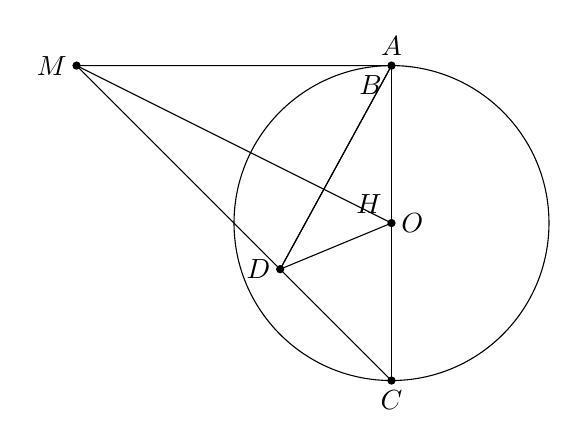
\begin{tikzpicture}[>=stealth, scale=1]
				\coordinate (O) at (0,0);
				\def\r{2}
				\draw (O) circle (\r);
				\coordinate (A) at (0,\r);
				\coordinate (C) at (0,-\r);
				\draw (A) -- (C);
				\coordinate (M) at (-4,\r);
				\draw (M) -- (A);
				\pgfmathsetmacro{\distM}{sqrt(16 + 4)}
				\pgfmathsetmacro{\angOM}{atan2(\r,-4)}
				\pgfmathsetmacro{\alphaVal}{acos(\r/\distM)}
				\coordinate (B) at ({\angOM - \alphaVal}:\r);
				\draw (M) -- (B);
				\draw (O) -- (B);
				\draw (O) -- (M);
				\draw (A) -- (B);
				\coordinate (H) at (intersection of A--B and M--O);
				\draw (M) -- (C);
				% D là điểm trên MC: vector MC = (4, -4)
				\coordinate (D) at (-1.414, -0.586);
				\draw (A) -- (D);
				\draw (H) -- (D);
				\draw (B) -- (D);
				\node at (O) [right] {$O$};
				\node at (A) [above] {$A$};
				\node at (C) [below] {$C$};
				\node at (M) [left] {$M$};
				\node at (B) [below left] {$B$};
				\node at (H) [above left] {$H$};
				\node at (D) [left] {$D$};
				\fill (O) circle (1.5pt) (A) circle (1.5pt) (C) circle (1.5pt) (M) circle (1.5pt) (B) circle (1.5pt) (H) circle (1.5pt) (D) circle (1.5pt);
			\end{tikzpicture}
		\end{center}
		\begin{enumerate}[a)]
			\item Vì $\widehat{ADC}$ là góc nội tiếp chắn nửa đường tròn đường kính $AC$ nên $\widehat{ADC} = 90^\circ \implies AD \perp MC \implies \widehat{ADM} = 90^\circ$.
			
			Vì $MA, MB$ là hai tiếp tuyến cắt nhau của $(O)$ nên $MA = MB$ và $OA = OB = R$, suy ra $MO$ là đường trung trực của $AB \implies MO \perp AB$ tại $H \implies \widehat{MHA} = 90^\circ$.
			
			Tứ giác $MDHA$ có $\widehat{ADM} = \widehat{MHA} = 90^\circ$, do đó hai đỉnh kề nhau $D$ và $H$ cùng nhìn đoạn $MA$ dưới góc vuông.
			
			Suy ra tứ giác $MDHA$ nội tiếp đường tròn đường kính $MA$.
			\item Vì $MA$ là tiếp tuyến tại $A$ của $(O)$ nên $MA \perp OA \implies \widehat{MAC} = 90^\circ$.
			
			Xét $\Delta MDA$ và $\Delta MAC$ có:
			$$\widehat{AMD}\text{ chung},\quad \widehat{MDA} = \widehat{MAC} = 90^\circ.$$
			Do đó $\Delta MDA \backsim \Delta MAC\text{ (g-g)}$, suy ra:
			$$\dfrac{MD}{MA} = \dfrac{MA}{MC} \implies MA^2 = MD \cdot MC. \quad (1)$$
			Xét tam giác vuông $MAO$ tại $A$ có đường cao $AH$, theo hệ thức lượng:
			$$MA^2 = MH \cdot MO. \quad (2)$$
			Từ $(1)$ và $(2)$ suy ra $MD \cdot MC = MH \cdot MO$.
			
			Từ $MD \cdot MC = MH \cdot MO \implies \dfrac{MH}{MC} = \dfrac{MD}{MO}$.
			
			Xét $\Delta MHD$ và $\Delta MCO$ có:
			$$\widehat{CMO}\text{ chung},\quad \dfrac{MH}{MC} = \dfrac{MD}{MO}.$$
			Do đó $\Delta MHD \backsim \Delta MCO\text{ (c-g-c)} \implies \widehat{MHD} = \widehat{MCO}$.
			
			Trong đường tròn $(O)$, hai góc nội tiếp $\widehat{MCO}$ (tức $\widehat{ACD}$) và $\widehat{ABD}$ cùng chắn cung $AD$ nên $\widehat{MCO} = \widehat{ABD}$.
			
			Suy ra $\widehat{MHD} = \widehat{DBA}$.
			\item Vì $MO \perp AB$ tại $H$ nên $\widehat{MHD} + \widehat{DHB} = 90^\circ$.
			
			Mà $\widehat{MHD} = \widehat{DBA}$ nên $\widehat{DBA} + \widehat{DHB} = 90^\circ$.
			
			Xét tam giác $HDB$ có tổng hai góc nhọn bằng $90^\circ$ nên góc còn lại $\widehat{HDB} = 90^\circ$.
			
			Khi $MA = 2R$:
			
			Tam giác $MAC$ vuông tại $A$ có $AC = 2R, MA = 2R$ nên $\Delta MAC$ vuông cân tại $A \implies \widehat{MCA} = 45^\circ$.
			
			Suy ra $\widehat{DBH} = \widehat{DCA} = 45^\circ$.
			
			Tam giác $HDB$ vuông tại $D$ có $\widehat{DBH} = 45^\circ$ nên $\Delta HDB$ vuông cân tại $D$.
			
			Kẻ $DQ \perp AB$ tại $Q$, khi đó $DQ$ vừa là đường cao vừa là trung tuyến ứng với cạnh huyền $HB$ của $\Delta HDB$:
			$$DQ = \dfrac{1}{2}HB.$$
			Trong tam giác vuông $MAO$ tại $A$ có đường cao $AH$:
			$$MO = \sqrt{OA^2 + MA^2} = \sqrt{R^2 + (2R)^2} = R\sqrt{5};$$
			$$AH = \dfrac{OA \cdot MA}{MO} = \dfrac{R \cdot 2R}{R\sqrt{5}} = \dfrac{2R}{\sqrt{5}}.$$
			Vì $H$ là trung điểm của $AB$ nên:
			$$HB = AH = \dfrac{2R}{\sqrt{5}},\quad AB = 2AH = \dfrac{4R}{\sqrt{5}}.$$
			Suy ra:
			$$DQ = \dfrac{1}{2}HB = \dfrac{R}{\sqrt{5}}.$$
			Diện tích tam giác $ABD$ là:
			$$S_{ABD} = \dfrac{1}{2} \cdot AB \cdot DQ = \dfrac{1}{2} \cdot \dfrac{4R}{\sqrt{5}} \cdot \dfrac{R}{\sqrt{5}} = \dfrac{2R^2}{5}.$$
			Vậy $S_{ABD} = \dfrac{2R^2}{5}$.
		\end{enumerate}
	}
\end{bt}
